\chapter{Results}

The solution quality and performance of the heuristic algorithm are primarily evaluated by comparing the implementation with an integer linear programming (ILP) model, described in AMPL and executed using CPLEX linear solver, herein simply referred to as \textit{ILP solutions}.\footnote{The full results, containing all input and output files, can be found in the following public \textit{GitHub} repository: \url{https://github.com/LMesaric/MSc-Thesis-FER-2022}.}
While the ILP can find optimal solutions for smaller instances, it is not scalable for larger instances.
Thus, the ILP was run with a maximal time limit and the suboptimal solutions obtained were used for comparison with the proposed heuristic algorithm.

All test scenarios used the same objective function weighting factors: $a_1 = 10^7$, $a_2 = 10^2$, $a_3 = 10^{-4}$.
As a part of the analysis, three different \textit{correction factor} ($\mathit{CF}$) values were used: $15\%$, $25\%$, $50\%$.
This was done to investigate the solution quality under increasing target water content.

Five randomly generated test instances were evaluated for every test scenario.
With seven sizes, two distributions over time (IA, MUOT), two distributions over fronts (NUOF, UOF), three correction factor values, and five instances for each combination, a total of 420 problem instances were used in the evaluation, with 60 instances for each scenario size.

Three different machines were used to find heuristic and ILP results presented in this chapter.
All used processors support dividing each physical core into two logical processors (threads).
Their hardware and operating system specifications are:
\begin{itemize}
    \item AMD Ryzen(TM) 7 5800H CPU at \SI{4.00}{\GHz} (8 cores, 16 threads),  \SI{16.00}{\giga\byte} DDR4 RAM, Windows~10 Home 64-bit,
    \item AMD Ryzen(TM) 9 3900X CPU at \SI{4.40}{\GHz} (12 cores, 24 threads), \SI{32.00}{\giga\byte} DDR4 RAM, Windows~10 Education 64-bit,
    \item Intel(R) Core(TM) i7-7700 at \SI{3.60}{\GHz} (4 cores, 8 threads),   \SI{16.00}{\giga\byte} DDR4 RAM, Windows~10 Pro 64-bit.
\end{itemize}


\section{Comparison of Heuristic and ILP Results}

Results are presented in Table~\ref{tbl:comparison-cf-15}, Table~\ref{tbl:comparison-cf-25}, and Table~\ref{tbl:comparison-cf-50}, one for each value of the correction factor.
Shown values are the arithmetic means for the five instances of the same test scenario.
They were rounded to the nearest integer as differences of less than one liter are considered negligible.
If the optimal solution was found for one or more instances, the scenario is marked with a single asterisk.
If the optimal solution was found for all five instances, the scenario is marked with a double asterisk.
The requirements for a solution to be considered optimal are explained in Section~\ref{sec:discussion}.

Because of the stark differences between the values of the weighting factors $a_1$, $a_2$, and $a_3$, for example, a solution which has a slightly better negative water surplus and a significantly worse minimal water surplus is still considered to be overall better.
Therefore, the solutions are effectively compared as tuples $(\!\mathit{WS_n}, \mathit{Z}, \mathit{WO})$.
The better of the two solutions for the same scenario is written in a bold font.

The differences between each of the three objectives are expressed in terms of the number of average-sized downloads (drops) of water, to put the results in perspective.
A positive value means the heuristic algorithm performed better with respect to the relevant objective.
The amount of water in an average-sized download depends on the instance size, specifically on the number of aircraft of each subtype.
It is calculated by dividing the estimated total water output of all aircraft with the estimated average number of downloads, using the data from Table~\ref{tbl:capacity-and-droprate}.
For example, if a heavy helicopter makes four flights, each lasting two hours, and performing on average four drops per hour, the estimated total number of drops it will make is $4 \cdot \SI{2}{\hour} \cdot \SI{4}{\per\hour} = 32$, and the estimated total water output is $32 \cdot \SI{4500}{\liter} = \SI{144000}{\liter}$.
For the test scenarios shown in Table~\ref{tbl:scenario-sizes}, the capacity of an average-sized download ranges between approximately \SI{2700}{\liter} and \SI{3000}{\liter}.

The ILP model was run on the machine with the i7-7700 CPU with a time limit of two hours, terminating early only if the optimal solution was found, which rarely happened.
The heuristic algorithm was executed on the machines with the 5800H and 3900X CPUs, using different hyperparameters.
For every test instance, up to 200 GRASP and 7\,000 local search iterations were executed.
The better of the two runs (for each instance) was selected as the heuristic solution presented in this paper.

\begin{landscape}
\begin{table}[htbp]
\footnotesize
\caption{Comparison of heuristic (H) and ILP results for $\mathit{CF} = 15\%$}
\label{tbl:comparison-cf-15}
\centering

\def\mygapstart{0mm}

\def\someoptimal{\makebox[0pt][l]{$^{\ast}$}}
\def\alloptimal{\makebox[0pt][l]{$^{\ast\ast}$}}

\newcommand{\twoline}[2]{\begin{tabular}[c]{@{}c@{}}#1 \\ #2\end{tabular}}
\newcommand{\diff}{\twoline{Deviation}{(no. of dls.)}}

\begin{tabular}{ll<{\hspace{\mygapstart}}*{4}{|rrr}}
\multicolumn{2}{c}{} & \multicolumn{3}{c}{NUOF + IA} & \multicolumn{3}{c}{NUOF + MUOT} & \multicolumn{3}{c}{UOF + IA} & \multicolumn{3}{c}{UOF + MUOT} \\ 
\cmidrule(lr){3-5} \cmidrule(lr){6-8} \cmidrule(lr){9-11} \cmidrule(lr){12-14}
{} & {} & H & ILP & \diff & H & ILP & \diff & H & ILP & \diff & H & ILP & \diff \\ \hline

\multirow{3}{*}{\rotatebox[origin=c]{90}{K07\_F02}}
& $\mathit{WS_n}$ & $-173$\someoptimal & $\pmb{-173}$\alloptimal & $0.000$ & $-238$\someoptimal & $\pmb{-235}$\alloptimal & $-0.001$ & $-189$\someoptimal & $\pmb{-189}$\alloptimal & $0.000$ & $\pmb{-30}$\alloptimal & $-30$\alloptimal & $0.000$ \\ 
& $\mathit{Z}$ & $-62$\someoptimal & $\pmb{-51}$\alloptimal & $-0.004$ & $-47$\someoptimal & $\pmb{-58}$\alloptimal & $0.004$ & $-83$\someoptimal & $\pmb{-59}$\alloptimal & $-0.008$ & $\pmb{171}$\alloptimal & $171$\alloptimal & $0.000$ \\ 
& $\mathit{WO}$ & $468188$\someoptimal & $\pmb{468607}$\alloptimal & $-0.140$ & $484432$\someoptimal & $\pmb{483953}$\alloptimal & $0.159$ & $468851$\someoptimal & $\pmb{464343}$\alloptimal & $1.503$ & $\pmb{428983}$\alloptimal & $427730$\alloptimal & $0.418$ \\ \hline

\multirow{3}{*}{\rotatebox[origin=c]{90}{K10\_F03}}
& $\mathit{WS_n}$ & $-133$\someoptimal & $\pmb{-98}$\alloptimal & $-0.012$ & $-126$\someoptimal & $\pmb{-37}$\alloptimal & $-0.031$ & $-208$\someoptimal & $\pmb{-136}$\alloptimal & $-0.025$ & $-168$\someoptimal & $\pmb{-90}$\someoptimal & $-0.028$ \\ 
& $\mathit{Z}$ & $7$\someoptimal & $\pmb{154}$\alloptimal & $-0.052$ & $-21$\someoptimal & $\pmb{111}$\alloptimal & $-0.047$ & $-29$\someoptimal & $\pmb{107}$\alloptimal & $-0.048$ & $-64$\someoptimal & $\pmb{54}$\someoptimal & $-0.042$ \\ 
& $\mathit{WO}$ & $687429$\someoptimal & $\pmb{685224}$\alloptimal & $0.783$ & $700775$\someoptimal & $\pmb{690004}$\alloptimal & $3.823$ & $678180$\someoptimal & $\pmb{677711}$\alloptimal & $0.166$ & $701048$\someoptimal & $\pmb{693559}$\someoptimal & $2.659$ \\ \hline

\multirow{3}{*}{\rotatebox[origin=c]{90}{K15\_F03}}
& $\mathit{WS_n}$ & $\pmb{0}$ & $0$ & $0.000$ & $\pmb{0}$ & $0$ & $0.000$ & $\pmb{0}$ & $0$ & $0.000$ & $\pmb{0}$ & $0$ & $0.000$ \\ 
& $\mathit{Z}$ & $\pmb{500}$ & $485$ & $0.005$ & $\pmb{550}$ & $485$ & $0.023$ & $\pmb{507}$ & $456$ & $0.018$ & $\pmb{554}$ & $413$ & $0.050$ \\ 
& $\mathit{WO}$ & $\pmb{954880}$ & $922474$ & $11.459$ & $\pmb{934539}$ & $932870$ & $0.590$ & $\pmb{938814}$ & $937418$ & $0.493$ & $\pmb{913906}$ & $895341$ & $6.565$ \\ \hline

\multirow{3}{*}{\rotatebox[origin=c]{90}{K20\_F04}}
& $\mathit{WS_n}$ & $\pmb{0}$ & $0$ & $0.000$ & $\pmb{-26}$ & $-26$ & $0.000$ & $\pmb{0}$ & $-63$ & $0.023$ & $\pmb{-44}$ & $-92$ & $0.018$ \\ 
& $\mathit{Z}$ & $\pmb{819}$ & $528$ & $0.108$ & $\pmb{465}$ & $182$ & $0.105$ & $\pmb{752}$ & $297$ & $0.169$ & $\pmb{515}$ & $132$ & $0.142$ \\ 
& $\mathit{WO}$ & $\pmb{1289480}$ & $1304870$ & $-5.715$ & $\pmb{1273218}$ & $1227526$ & $16.968$ & $\pmb{1325138}$ & $1292050$ & $12.288$ & $\pmb{1274888}$ & $1254996$ & $7.387$ \\ \hline

\multirow{3}{*}{\rotatebox[origin=c]{90}{K25\_F04}}
& $\mathit{WS_n}$ & $\pmb{0}$ & $-1004$ & $0.370$ & $\pmb{0}$ & $-37$ & $0.013$ & $\pmb{0}$ & $0$ & $0.000$ & $\pmb{0}$ & $-246$ & $0.091$ \\ 
& $\mathit{Z}$ & $\pmb{998}$ & $-450$ & $0.534$ & $\pmb{1031}$ & $234$ & $0.294$ & $\pmb{1250}$ & $616$ & $0.234$ & $\pmb{988}$ & $81$ & $0.335$ \\ 
& $\mathit{WO}$ & $\pmb{1557007}$ & $1556972$ & $0.013$ & $\pmb{1624811}$ & $1624768$ & $0.016$ & $\pmb{1625807}$ & $1594114$ & $11.688$ & $\pmb{1653663}$ & $1573720$ & $29.482$ \\ \hline

\multirow{3}{*}{\rotatebox[origin=c]{90}{K30\_F05}}
& $\mathit{WS_n}$ & $\pmb{0}$ & $-6531$ & $2.389$ & $\pmb{0}$ & $-2345$ & $0.858$ & $\pmb{0}$ & $-2362$ & $0.864$ & $\pmb{0}$ & $-1614$ & $0.590$ \\ 
& $\mathit{Z}$ & $\pmb{1247}$ & $-632$ & $0.687$ & $\pmb{1122}$ & $-571$ & $0.619$ & $\pmb{1087}$ & $-627$ & $0.627$ & $\pmb{1024}$ & $-479$ & $0.550$ \\ 
& $\mathit{WO}$ & $\pmb{1935023}$ & $1751826$ & $67.010$ & $\pmb{1876768}$ & $1744786$ & $48.277$ & $\pmb{1907201}$ & $1714092$ & $70.636$ & $\pmb{1889009}$ & $1765286$ & $45.256$ \\ \hline

\multirow{3}{*}{\rotatebox[origin=c]{90}{K35\_F05}}
& $\mathit{WS_n}$ & $\pmb{0}$ & $-18018$ & $6.573$ & $\pmb{0}$ & $-5629$ & $2.054$ & $\pmb{0}$ & $-8425$ & $3.073$ & $\pmb{0}$ & $-6110$ & $2.229$ \\ 
& $\mathit{Z}$ & $\pmb{910}$ & $-2455$ & $1.228$ & $\pmb{1010}$ & $-901$ & $0.697$ & $\pmb{1201}$ & $-1953$ & $1.151$ & $\pmb{1220}$ & $-1245$ & $0.899$ \\ 
& $\mathit{WO}$ & $\pmb{2085463}$ & $1777452$ & $112.356$ & $\pmb{2087712}$ & $2017826$ & $25.493$ & $\pmb{2363235}$ & $2211200$ & $55.459$ & $\pmb{2284475}$ & $2027012$ & $93.917$ \\

\end{tabular}
\end{table}
\end{landscape}

\begin{landscape}
\begin{table}[htbp]
\footnotesize
\caption{Comparison of heuristic (H) and ILP results for $\mathit{CF} = 25\%$}
\label{tbl:comparison-cf-25}
\centering

\def\mygapstart{0mm}

\def\someoptimal{\makebox[0pt][l]{$^{\ast}$}}
\def\alloptimal{\makebox[0pt][l]{$^{\ast\ast}$}}

\newcommand{\twoline}[2]{\begin{tabular}[c]{@{}c@{}}#1 \\ #2\end{tabular}}
\newcommand{\diff}{\twoline{Deviation}{(no. of dls.)}}

\begin{tabular}{ll<{\hspace{\mygapstart}}*{4}{|rrr}}
\multicolumn{2}{c}{} & \multicolumn{3}{c}{NUOF + IA} & \multicolumn{3}{c}{NUOF + MUOT} & \multicolumn{3}{c}{UOF + IA} & \multicolumn{3}{c}{UOF + MUOT} \\ 
\cmidrule(lr){3-5} \cmidrule(lr){6-8} \cmidrule(lr){9-11} \cmidrule(lr){12-14}
{} & {} & H & ILP & \diff & H & ILP & \diff & H & ILP & \diff & H & ILP & \diff \\ \hline

\multirow{3}{*}{\rotatebox[origin=c]{90}{K07\_F02}}
& $\mathit{WS_n}$ & $-797$\someoptimal & $\pmb{-776}$\alloptimal & $-0.007$ & $\pmb{-871}$\alloptimal & $-871$\alloptimal & $0.000$ & $-967$\someoptimal & $\pmb{-780}$\alloptimal & $-0.062$ & $-912$\someoptimal & $\pmb{-903}$\alloptimal & $-0.003$ \\ 
& $\mathit{Z}$ & $-400$\someoptimal & $\pmb{-332}$\alloptimal & $-0.023$ & $\pmb{-378}$\alloptimal & $-378$\alloptimal & $0.000$ & $-525$\someoptimal & $\pmb{-419}$\alloptimal & $-0.035$ & $-349$\someoptimal & $\pmb{-349}$\alloptimal & $0.000$ \\ 
& $\mathit{WO}$ & $466143$\someoptimal & $\pmb{437246}$\alloptimal & $9.633$ & $\pmb{485478}$\alloptimal & $483170$\alloptimal & $0.769$ & $450239$\someoptimal & $\pmb{427062}$\alloptimal & $7.726$ & $487367$\someoptimal & $\pmb{474622}$\alloptimal & $4.248$ \\ \hline 

\multirow{3}{*}{\rotatebox[origin=c]{90}{K10\_F03}}
& $\mathit{WS_n}$ & $-479$\someoptimal & $\pmb{-271}$\alloptimal & $-0.074$ & $-244$\someoptimal & $\pmb{-219}$\someoptimal & $-0.009$ & $-638$\someoptimal & $\pmb{-622}$\someoptimal & $-0.005$ & $-292$\someoptimal & $\pmb{-289}$\someoptimal & $-0.001$ \\ 
& $\mathit{Z}$ & $-219$\someoptimal & $\pmb{-69}$\alloptimal & $-0.053$ & $-125$\someoptimal & $\pmb{-79}$\someoptimal & $-0.017$ & $-326$\someoptimal & $\pmb{-283}$\someoptimal & $-0.015$ & $-180$\someoptimal & $\pmb{-180}$\someoptimal & $0.000$ \\ 
& $\mathit{WO}$ & $689887$\someoptimal & $\pmb{667833}$\alloptimal & $7.829$ & $695754$\someoptimal & $\pmb{686653}$\someoptimal & $3.231$ & $687891$\someoptimal & $\pmb{670438}$\someoptimal & $6.196$ & $697977$\someoptimal & $\pmb{697431}$\someoptimal & $0.194$ \\ \hline 

\multirow{3}{*}{\rotatebox[origin=c]{90}{K15\_F03}}
& $\mathit{WS_n}$ & $\pmb{-4}$ & $-81$ & $0.027$ & $\pmb{-60}$ & $-378$ & $0.112$ & $\pmb{-53}$ & $-74$ & $0.007$ & $\pmb{-79}$ & $-757$ & $0.239$ \\ 
& $\mathit{Z}$ & $\pmb{286}$ & $163$ & $0.043$ & $\pmb{296}$ & $73$ & $0.079$ & $\pmb{201}$ & $92$ & $0.039$ & $\pmb{236}$ & $-336$ & $0.202$ \\ 
& $\mathit{WO}$ & $\pmb{974851}$ & $943844$ & $10.965$ & $\pmb{931316}$ & $921445$ & $3.491$ & $\pmb{935915}$ & $961386$ & $-9.007$ & $\pmb{927291}$ & $905444$ & $7.726$ \\ \hline 

\multirow{3}{*}{\rotatebox[origin=c]{90}{K20\_F04}}
& $\mathit{WS_n}$ & $\pmb{0}$ & $-580$ & $0.215$ & $\pmb{-44}$ & $-771$ & $0.270$ & $\pmb{0}$ & $-515$ & $0.191$ & $\pmb{-73}$ & $-708$ & $0.236$ \\ 
& $\mathit{Z}$ & $\pmb{501}$ & $-96$ & $0.222$ & $\pmb{296}$ & $-418$ & $0.265$ & $\pmb{490}$ & $-213$ & $0.261$ & $\pmb{297}$ & $-235$ & $0.198$ \\ 
& $\mathit{WO}$ & $\pmb{1293201}$ & $1267246$ & $9.639$ & $\pmb{1260252}$ & $1193833$ & $24.666$ & $\pmb{1294392}$ & $1276368$ & $6.694$ & $\pmb{1266846}$ & $1177696$ & $33.107$ \\ \hline 

\multirow{3}{*}{\rotatebox[origin=c]{90}{K25\_F04}}
& $\mathit{WS_n}$ & $\pmb{0}$ & $-6396$ & $2.359$ & $\pmb{0}$ & $-3707$ & $1.367$ & $\pmb{0}$ & $-2142$ & $0.790$ & $\pmb{0}$ & $-2334$ & $0.861$ \\ 
& $\mathit{Z}$ & $\pmb{687}$ & $-2282$ & $1.095$ & $\pmb{438}$ & $-982$ & $0.524$ & $\pmb{933}$ & $-637$ & $0.579$ & $\pmb{714}$ & $-1137$ & $0.683$ \\ 
& $\mathit{WO}$ & $\pmb{1624734}$ & $1596726$ & $10.329$ & $\pmb{1615536}$ & $1525710$ & $33.127$ & $\pmb{1620544}$ & $1441906$ & $65.881$ & $\pmb{1620279}$ & $1519582$ & $37.136$ \\ \hline 

\multirow{3}{*}{\rotatebox[origin=c]{90}{K30\_F05}}
& $\mathit{WS_n}$ & $\pmb{0}$ & $-10615$ & $3.883$ & $\pmb{0}$ & $-22177$ & $8.112$ & $\pmb{0}$ & $-11170$ & $4.086$ & $\pmb{0}$ & $-14438$ & $5.281$ \\ 
& $\mathit{Z}$ & $\pmb{869}$ & $-2040$ & $1.064$ & $\pmb{770}$ & $-2247$ & $1.104$ & $\pmb{708}$ & $-1319$ & $0.741$ & $\pmb{680}$ & $-1850$ & $0.925$ \\ 
& $\mathit{WO}$ & $\pmb{1897405}$ & $1780406$ & $42.796$ & $\pmb{1914978}$ & $1728888$ & $68.068$ & $\pmb{1892579}$ & $1638394$ & $92.976$ & $\pmb{1880980}$ & $1574298$ & $112.179$ \\ \hline 

\multirow{3}{*}{\rotatebox[origin=c]{90}{K35\_F05}}
& $\mathit{WS_n}$ & $\pmb{0}$ & $-27702$ & $10.105$ & $\pmb{-7}$ & $-17986$ & $6.558$ & $\pmb{0}$ & $-45151$ & $16.470$ & $\pmb{0}$ & $-19260$ & $7.026$ \\ 
& $\mathit{Z}$ & $\pmb{665}$ & $-4230$ & $1.786$ & $\pmb{758}$ & $-2279$ & $1.108$ & $\pmb{845}$ & $-3438$ & $1.562$ & $\pmb{916}$ & $-1792$ & $0.988$ \\ 
& $\mathit{WO}$ & $\pmb{2059599}$ & $1793304$ & $97.139$ & $\pmb{2109832}$ & $1859236$ & $91.412$ & $\pmb{2379209}$ & $2038154$ & $124.410$ & $\pmb{2307628}$ & $2057578$ & $91.213$ \\ 

\end{tabular}
\end{table}
\end{landscape}

\begin{landscape}
\begin{table}[htbp]
\footnotesize
\caption{Comparison of heuristic (H) and ILP results for $\mathit{CF} = 50\%$}
\label{tbl:comparison-cf-50}
\centering

\def\mygapstart{0mm}

\def\someoptimal{\makebox[0pt][l]{$^{\ast}$}}
\def\alloptimal{\makebox[0pt][l]{$^{\ast\ast}$}}

\newcommand{\twoline}[2]{\begin{tabular}[c]{@{}c@{}}#1 \\ #2\end{tabular}}
\newcommand{\diff}{\twoline{Deviation}{(no. of dls.)}}

\begin{tabular}{ll<{\hspace{\mygapstart}}*{4}{|rrr}}
\multicolumn{2}{c}{} & \multicolumn{3}{c}{NUOF + IA} & \multicolumn{3}{c}{NUOF + MUOT} & \multicolumn{3}{c}{UOF + IA} & \multicolumn{3}{c}{UOF + MUOT} \\ 
\cmidrule(lr){3-5} \cmidrule(lr){6-8} \cmidrule(lr){9-11} \cmidrule(lr){12-14}
{} & {} & H & ILP & \diff & H & ILP & \diff & H & ILP & \diff & H & ILP & \diff \\ \hline

\multirow{3}{*}{\rotatebox[origin=c]{90}{K07\_F02}}
& $\mathit{WS_n}$ & $-2989$\someoptimal & $\pmb{-2883}$\alloptimal & $-0.035$ & $-2012$\someoptimal & $\pmb{-1844}$\alloptimal & $-0.056$ & $-2301$\someoptimal & $\pmb{-2274}$\alloptimal & $-0.009$ & $\pmb{-1823}$\alloptimal & $-1823$\alloptimal & $0.000$ \\ 
& $\mathit{Z}$ & $-1019$\someoptimal & $\pmb{-973}$\alloptimal & $-0.015$ & $-763$\someoptimal & $\pmb{-881}$\alloptimal & $0.039$ & $-1318$\someoptimal & $\pmb{-1318}$\alloptimal & $0.000$ & $\pmb{-1015}$\alloptimal & $-1015$\alloptimal & $0.000$ \\ 
& $\mathit{WO}$ & $449896$\someoptimal & $\pmb{442592}$\alloptimal & $2.435$ & $493192$\someoptimal & $\pmb{487790}$\alloptimal & $1.801$ & $442313$\someoptimal & $\pmb{438901}$\alloptimal & $1.137$ & $\pmb{491523}$\alloptimal & $491225$\alloptimal & $0.099$ \\ \hline 

\multirow{3}{*}{\rotatebox[origin=c]{90}{K10\_F03}}
& $\mathit{WS_n}$ & $\pmb{-896}$\someoptimal & $-1127$\someoptimal & $0.082$ & $\pmb{-2854}$ & $-2948$\someoptimal & $0.033$ & $\pmb{-1542}$ & $-2207$\someoptimal & $0.236$ & $\pmb{-4599}$ & $-6554$ & $0.694$ \\ 
& $\mathit{Z}$ & $\pmb{-444}$\someoptimal & $-536$\someoptimal & $0.033$ & $\pmb{-1205}$ & $-1225$\someoptimal & $0.007$ & $\pmb{-546}$ & $-777$\someoptimal & $0.082$ & $\pmb{-1698}$ & $-1927$ & $0.082$ \\ 
& $\mathit{WO}$ & $\pmb{720051}$\someoptimal & $716686$\someoptimal & $1.195$ & $\pmb{652713}$ & $654070$\someoptimal & $-0.482$ & $\pmb{710147}$ & $707986$\someoptimal & $0.767$ & $\pmb{641558}$ & $635346$ & $2.205$ \\ \hline 

\multirow{3}{*}{\rotatebox[origin=c]{90}{K15\_F03}}
& $\mathit{WS_n}$ & $\pmb{-2542}$ & $-2973$\someoptimal & $0.152$ & $\pmb{-2721}$ & $-4002$ & $0.453$ & $\pmb{-3527}$ & $-4486$ & $0.339$ & $\pmb{-3573}$ & $-5769$ & $0.777$ \\ 
& $\mathit{Z}$ & $\pmb{-1296}$ & $-1444$\someoptimal & $0.052$ & $\pmb{-1271}$ & $-1745$ & $0.168$ & $\pmb{-1446}$ & $-1606$ & $0.057$ & $\pmb{-1232}$ & $-1821$ & $0.208$ \\ 
& $\mathit{WO}$ & $\pmb{980092}$ & $975986$\someoptimal & $1.452$ & $\pmb{914063}$ & $897083$ & $6.004$ & $\pmb{977230}$ & $968173$ & $3.203$ & $\pmb{900147}$ & $910705$ & $-3.734$ \\ \hline 

\multirow{3}{*}{\rotatebox[origin=c]{90}{K20\_F04}}
& $\mathit{WS_n}$ & $\pmb{-1715}$ & $-10184$ & $3.145$ & $\pmb{-1470}$ & $-9855$ & $3.114$ & $\pmb{-1466}$ & $-7625$ & $2.287$ & $\pmb{-1708}$ & $-13600$ & $4.416$ \\ 
& $\mathit{Z}$ & $\pmb{-777}$ & $-2880$ & $0.781$ & $\pmb{-588}$ & $-2921$ & $0.866$ & $\pmb{-353}$ & $-2185$ & $0.680$ & $\pmb{-790}$ & $-1988$ & $0.445$ \\ 
& $\mathit{WO}$ & $\pmb{1210731}$ & $1135203$ & $28.049$ & $\pmb{1251442}$ & $1237540$ & $5.163$ & $\pmb{1246658}$ & $1205878$ & $15.144$ & $\pmb{1239359}$ & $1197545$ & $15.528$ \\ \hline 

\multirow{3}{*}{\rotatebox[origin=c]{90}{K25\_F04}}
& $\mathit{WS_n}$ & $\pmb{-152}$ & $-13990$ & $5.104$ & $\pmb{-88}$ & $-18996$ & $6.973$ & $\pmb{-656}$ & $-37551$ & $13.607$ & $\pmb{-63}$ & $-13246$ & $4.862$ \\ 
& $\mathit{Z}$ & $\pmb{-55}$ & $-3156$ & $1.144$ & $\pmb{86}$ & $-3476$ & $1.314$ & $\pmb{-120}$ & $-4562$ & $1.639$ & $\pmb{190}$ & $-2907$ & $1.142$ \\ 
& $\mathit{WO}$ & $\pmb{1611245}$ & $1606310$ & $1.820$ & $\pmb{1605835}$ & $1515948$ & $33.150$ & $\pmb{1666759}$ & $1472142$ & $71.774$ & $\pmb{1629678}$ & $1546952$ & $30.509$ \\ \hline 

\multirow{3}{*}{\rotatebox[origin=c]{90}{K30\_F05}}
& $\mathit{WS_n}$ & $\pmb{-470}$ & $-89250$ & $32.474$ & $\pmb{-284}$ & $-26813$ & $9.704$ & $\pmb{-625}$ & $-62326$ & $22.569$ & $\pmb{-595}$ & $-61670$ & $22.340$ \\ 
& $\mathit{Z}$ & $\pmb{-24}$ & $-6762$ & $2.465$ & $\pmb{-106}$ & $-4317$ & $1.541$ & $\pmb{-365}$ & $-5088$ & $1.728$ & $\pmb{-159}$ & $-4129$ & $1.452$ \\ 
& $\mathit{WO}$ & $\pmb{1937631}$ & $1689280$ & $90.842$ & $\pmb{1927256}$ & $1767732$ & $58.351$ & $\pmb{1971345}$ & $1655500$ & $115.530$ & $\pmb{2044985}$ & $1749104$ & $108.228$ \\ \hline 

\multirow{3}{*}{\rotatebox[origin=c]{90}{K35\_F05}}
& $\mathit{WS_n}$ & $\pmb{-968}$ & $-134787$ & $48.814$ & $\pmb{-175}$ & $-124334$ & $45.291$ & $\pmb{-696}$ & $-142156$ & $51.602$ & $\pmb{-365}$ & $-132965$ & $48.370$ \\ 
& $\mathit{Z}$ & $\pmb{-561}$ & $-8363$ & $2.846$ & $\pmb{57}$ & $-6597$ & $2.427$ & $\pmb{-273}$ & $-5479$ & $1.899$ & $\pmb{-158}$ & $-4322$ & $1.519$ \\ 
& $\mathit{WO}$ & $\pmb{2121506}$ & $1819684$ & $110.099$ & $\pmb{2148979}$ & $1785340$ & $132.648$ & $\pmb{2252157}$ & $1659594$ & $216.155$ & $\pmb{2162483}$ & $1690788$ & $172.065$ \\ 

\end{tabular}
\end{table}
\end{landscape}



\section{Comparison with Extended Execution Time}

In order to more accurately assess the quality of the solutions found by the heuristic algorithm for larger instances, CPLEX solver was used on ten randomly selected test instances, with effectively six times longer execution time.
This was achieved by executing instances with a time limit of six hours, which is three times longer than for previous instances, and using a CPU with double the physical and logical core count (Ryzen 7 5800H).
Even though a laptop was used, and the CPU usage was consistently very high (often staying at $100\%$ for a short time), there were no signs of overheating or CPU throttling, with temperatures staying well below \SI{65}{\degreeCelsius}, and the CPU clock speed not dropping under 3.90~GHz.

The test instances were randomly picked by hand.
Two instances were selected from each test scenario size with 15 or more aircraft (Table~\ref{tbl:scenario-sizes}), one with $\mathit{CF} = 15\%$, and the other with $\mathit{CF} = 50\%$.
Different distributions of the target water content were sampled, to keep the scenarios varied.

The results are presented in Table~\ref{tbl:comparison-extended}.
These values are for single instances, and not average values of five instances.

\begin{table}[htbp]
\footnotesize
\caption{Comparison of heuristic (H) and ILP results with extended execution time}
\label{tbl:comparison-extended}
\centering

\def\mygapstart{2mm}
\def\mygapmid{4mm}

\newcommand{\twoline}[2]{\begin{tabular}[c]{@{}c@{}}#1 \\ #2\end{tabular}}
\newcommand{\diff}{\twoline{Deviation}{(no. of dls.)}}

\begin{tabular}{
    ll
    <{\hspace{\mygapstart}}|>{\hspace{\mygapstart}}
    *3r
    <{\hspace{\mygapmid}}|>{\hspace{\mygapmid}}
    *3r
}
\multicolumn{2}{c}{} & \multicolumn{3}{c}{$\mathit{CF} = 15\%$} & \multicolumn{3}{c}{$\mathit{CF} = 50\%$} \\ 
\cmidrule(l{\mygapstart}r{\mygapmid}){3-5} \cmidrule(l{\mygapmid}r){6-8}
{} & {} & H & ILP & \diff & H & ILP & \diff \\ \hline

\multirow{3}{*}{\rotatebox[origin=c]{90}{K15\_F03}}
& $\mathit{WS_n}$ & $0$ & $\pmb{0}$ & $0.00$ & $\pmb{-1357}$ & $-1653$ & $0.10$ \\ 
& $\mathit{Z}$ & $564$ & $\pmb{638}$ & $-0.03$ & $\pmb{-545}$ & $-545$ & $0.00$ \\ 
& $\mathit{WO}$ & $940252$ & $\pmb{932840}$ & $2.62$ & $\pmb{833730}$ & $830704$ & $1.07$ \\ \hline

\multirow{3}{*}{\rotatebox[origin=c]{90}{K20\_F04}}
& $\mathit{WS_n}$ & $-131$ & $\pmb{0}$ & $-0.05$ & $\pmb{-978}$ & $-4868$ & $1.44$ \\ 
& $\mathit{Z}$ & $-131$ & $\pmb{41}$ & $-0.06$ & $\pmb{-433}$ & $-2174$ & $0.65$ \\ 
& $\mathit{WO}$ & $1186142$ & $\pmb{1208480}$ & $-8.30$ & $\pmb{1133633}$ & $1142120$ & $-3.15$ \\ \hline

\multirow{3}{*}{\rotatebox[origin=c]{90}{K25\_F04}}
& $\mathit{WS_n}$ & $\pmb{0}$ & $0$ & $0.00$ & $\pmb{0}$ & $-124$ & $0.05$ \\ 
& $\mathit{Z}$ & $\pmb{1120}$ & $582$ & $0.20$ & $\pmb{161}$ & $-124$ & $0.11$ \\ 
& $\mathit{WO}$ & $\pmb{1532352}$ & $1579490$ & $-17.38$ & $\pmb{1427212}$ & $1507580$ & $-29.64$ \\ \hline

\multirow{3}{*}{\rotatebox[origin=c]{90}{K30\_F05}}
& $\mathit{WS_n}$ & $\pmb{0}$ & $0$ & $0.00$ & $\pmb{0}$ & $-37635$ & $13.77$ \\ 
& $\mathit{Z}$ & $\pmb{1136}$ & $775$ & $0.13$ & $\pmb{12}$ & $-4960$ & $1.82$ \\ 
& $\mathit{WO}$ & $\pmb{1935784}$ & $1959720$ & $-8.76$ & $\pmb{2162213}$ & $2041240$ & $44.25$ \\ \hline

\multirow{3}{*}{\rotatebox[origin=c]{90}{K35\_F05}}
& $\mathit{WS_n}$ & $\pmb{0}$ & $0$ & $0.00$ & $\pmb{-378}$ & $-16843$ & $6.01$ \\ 
& $\mathit{Z}$ & $\pmb{165}$ & $31$ & $0.05$ & $\pmb{-244}$ & $-4000$ & $1.37$ \\ 
& $\mathit{WO}$ & $\pmb{1916688}$ & $1918110$ & $-0.52$ & $\pmb{2031193}$ & $1888430$ & $52.08$ \\ 
\end{tabular}
\end{table}



\section{Comparison of GRASP Phases}

The elapsed real time per GRASP iteration, measured in seconds, is shown in Table~\ref{tbl:iteration-time}.
Execution times for the randomized greedy algorithm and local search are also shown.
Their sum is approximately equal to the duration of a GRASP iteration.

These arithmetic means and standard deviations were calculated based on 12\,000 iterations for each test scenario size, i.e., a total of 84\,000 GRASP iterations were used.
The results are not divided based on the test scenario type like in previous tables as there were no noticeable differences in execution time.
Instead, measurements are only grouped based on the size of the scenario.

Only the results from the machine with the 3900X CPU were used, to keep measurements consistent.
The 3900X machine has 12 physical cores, and the heuristic algorithm was executed with 20 worker threads.
This means that Simultaneous Multithreading\footnote{AMD's equivalent of Intel's proprietary Hyper-Threading Technology.} was extensively used, and uneven thread scheduling could explain the approximately $10\%$ standard deviation with respect to iteration duration.

A fixed number of 7\,000 local search iterations was used for these measurements.
While that is reasonable for larger instances, the smaller ones typically converge much sooner.
For example, scenarios of size K10\_F03 could easily be executed within one second without the solution quality being noticeably diminished.

\begin{table}[htbp]
\sisetup{separate-uncertainty}
\footnotesize
\caption{Execution times for a GRASP iteration, divided into phases}
\label{tbl:iteration-time}
\centering

\begin{tabular}
  {
    l|
    S[table-format = 2.3(3)]
    S[table-format = 1.3(3)]
    S[table-format = 1.3(3)]
  }
\multicolumn{1}{c}{} & \multicolumn{3}{c}{Elapsed real time per GRASP iteration (\si{s})} \\
\cmidrule(lr){2-4}
Instance & \multicolumn{1}{c}{GRASP} & {Randomized greedy} & {Local search} \\
\midrule
K07\_F02 &  1.230(162)  & 0.008(1)   & 1.223(162)  \\
K10\_F03 &  2.630(343)  & 0.052(6)   & 2.578(344)  \\
K15\_F03 &  3.126(331)  & 0.150(15)  & 2.976(332)  \\
K20\_F04 &  5.809(551)  & 0.723(50)  & 5.086(550)  \\
K25\_F04 &  7.032(717)  & 1.321(83)  & 5.711(703)  \\
K30\_F05 & 12.439(914)  & 3.636(292) & 8.804(878)  \\
K35\_F05 & 14.644(1078) & 5.464(418) & 9.179(973)  \\
\end{tabular}
\end{table}


\begin{landscape}
\begin{table}[htbp]
\footnotesize
\caption{Comparison of randomized greedy (RG) and local search (LS) results for $\mathit{CF} = 50\%$}
\label{tbl:comparison-greedy-ls-50}
\centering

\def\mygapstart{0mm}

\def\someoptimal{\makebox[0pt][l]{$^{\ast}$}}
\def\alloptimal{\makebox[0pt][l]{$^{\ast\ast}$}}

\newcommand{\twoline}[2]{\begin{tabular}[c]{@{}c@{}}#1 \\ #2\end{tabular}}
\newcommand{\diff}{\twoline{Deviation}{(no. of dls.)}}

\begin{tabular}{ll<{\hspace{\mygapstart}}*{4}{|rrr}}
\multicolumn{2}{c}{} & \multicolumn{3}{c}{NUOF + IA} & \multicolumn{3}{c}{NUOF + MUOT} & \multicolumn{3}{c}{UOF + IA} & \multicolumn{3}{c}{UOF + MUOT} \\ 
\cmidrule(lr){3-5} \cmidrule(lr){6-8} \cmidrule(lr){9-11} \cmidrule(lr){12-14}
{} & {} & LS & RG & \diff & LS & RG & \diff & LS & RG & \diff & LS & RG & \diff \\ \hline

\multirow{3}{*}{\rotatebox[origin=c]{90}{K07\_F02}}
& $\mathit{WS_n}$ & $\pmb{-2989}$\someoptimal & $-6748$ & $1.253$ & $\pmb{-2012}$\someoptimal & $-4475$ & $0.821$ & $\pmb{-2301}$\someoptimal & $-4148$ & $0.616$ & $\pmb{-1823}$\alloptimal & $-4099$ & $0.759$ \\ 
& $\mathit{Z}$ & $\pmb{-1019}$\someoptimal & $-1853$ & $0.278$ & $\pmb{-763}$\someoptimal & $-1372$ & $0.203$ & $\pmb{-1318}$\someoptimal & $-1442$ & $0.041$ & $\pmb{-1015}$\alloptimal & $-1835$ & $0.274$ \\ 
& $\mathit{WO}$ & $\pmb{449896}$\someoptimal & $451482$ & $-0.529$ & $\pmb{493192}$\someoptimal & $491596$ & $0.532$ & $\pmb{442313}$\someoptimal & $439821$ & $0.830$ & $\pmb{491523}$\alloptimal & $491268$ & $0.085$ \\ \hline 
\multirow{3}{*}{\rotatebox[origin=c]{90}{K10\_F03}}
& $\mathit{WS_n}$ & $\pmb{-896}$\someoptimal & $-4834$ & $1.398$ & $\pmb{-2854}$ & $-8419$ & $1.975$ & $\pmb{-1542}$ & $-6776$ & $1.858$ & $\pmb{-4599}$ & $-12429$ & $2.779$ \\ 
& $\mathit{Z}$ & $\pmb{-444}$\someoptimal & $-1286$ & $0.299$ & $\pmb{-1205}$ & $-1932$ & $0.258$ & $\pmb{-546}$ & $-1659$ & $0.395$ & $\pmb{-1698}$ & $-1993$ & $0.105$ \\ 
& $\mathit{WO}$ & $\pmb{720051}$\someoptimal & $713320$ & $2.389$ & $\pmb{652713}$ & $649593$ & $1.108$ & $\pmb{710147}$ & $698928$ & $3.982$ & $\pmb{641558}$ & $644659$ & $-1.101$ \\ \hline 

\multirow{3}{*}{\rotatebox[origin=c]{90}{K15\_F03}}
& $\mathit{WS_n}$ & $\pmb{-2542}$ & $-8575$ & $2.133$ & $\pmb{-2721}$ & $-8024$ & $1.875$ & $\pmb{-3527}$ & $-9681$ & $2.176$ & $\pmb{-3573}$ & $-9844$ & $2.218$ \\ 
& $\mathit{Z}$ & $\pmb{-1296}$ & $-3049$ & $0.620$ & $\pmb{-1271}$ & $-2618$ & $0.476$ & $\pmb{-1446}$ & $-2890$ & $0.511$ & $\pmb{-1232}$ & $-2462$ & $0.435$ \\ 
& $\mathit{WO}$ & $\pmb{980092}$ & $965535$ & $5.148$ & $\pmb{914063}$ & $886811$ & $9.637$ & $\pmb{977230}$ & $968692$ & $3.019$ & $\pmb{900147}$ & $893642$ & $2.300$ \\ \hline 

\multirow{3}{*}{\rotatebox[origin=c]{90}{K20\_F04}}
& $\mathit{WS_n}$ & $\pmb{-1715}$ & $-8449$ & $2.501$ & $\pmb{-1470}$ & $-8624$ & $2.657$ & $\pmb{-1466}$ & $-6005$ & $1.685$ & $\pmb{-1708}$ & $-8230$ & $2.422$ \\ 
& $\mathit{Z}$ & $\pmb{-777}$ & $-2203$ & $0.530$ & $\pmb{-588}$ & $-2701$ & $0.785$ & $\pmb{-353}$ & $-2054$ & $0.632$ & $\pmb{-790}$ & $-2021$ & $0.457$ \\ 
& $\mathit{WO}$ & $\pmb{1210731}$ & $1194753$ & $5.934$ & $\pmb{1251442}$ & $1235285$ & $6.000$ & $\pmb{1246658}$ & $1231172$ & $5.751$ & $\pmb{1239359}$ & $1229243$ & $3.757$ \\ \hline 

\multirow{3}{*}{\rotatebox[origin=c]{90}{K25\_F04}}
& $\mathit{WS_n}$ & $\pmb{-152}$ & $-6338$ & $2.282$ & $\pmb{-88}$ & $-3680$ & $1.325$ & $\pmb{-656}$ & $-2845$ & $0.808$ & $\pmb{-63}$ & $-1629$ & $0.577$ \\ 
& $\mathit{Z}$ & $\pmb{-55}$ & $-2274$ & $0.818$ & $\pmb{86}$ & $-1380$ & $0.541$ & $\pmb{-120}$ & $-1045$ & $0.341$ & $\pmb{190}$ & $-778$ & $0.357$ \\ 
& $\mathit{WO}$ & $\pmb{1611245}$ & $1597549$ & $5.051$ & $\pmb{1605835}$ & $1588078$ & $6.549$ & $\pmb{1666759}$ & $1646783$ & $7.367$ & $\pmb{1629678}$ & $1608702$ & $7.736$ \\ \hline 

\multirow{3}{*}{\rotatebox[origin=c]{90}{K30\_F05}}
& $\mathit{WS_n}$ & $\pmb{-470}$ & $-6043$ & $2.038$ & $\pmb{-284}$ & $-4616$ & $1.585$ & $\pmb{-625}$ & $-6923$ & $2.304$ & $\pmb{-595}$ & $-5813$ & $1.909$ \\ 
& $\mathit{Z}$ & $\pmb{-24}$ & $-2272$ & $0.822$ & $\pmb{-106}$ & $-1251$ & $0.419$ & $\pmb{-365}$ & $-1855$ & $0.545$ & $\pmb{-159}$ & $-1537$ & $0.504$ \\ 
& $\mathit{WO}$ & $\pmb{1937631}$ & $1889475$ & $17.615$ & $\pmb{1927256}$ & $1856982$ & $25.705$ & $\pmb{1971345}$ & $1943905$ & $10.037$ & $\pmb{2044985}$ & $1997203$ & $17.478$ \\ \hline 

\multirow{3}{*}{\rotatebox[origin=c]{90}{K35\_F05}}
& $\mathit{WS_n}$ & $\pmb{-968}$ & $-12209$ & $4.100$ & $\pmb{-175}$ & $-4945$ & $1.740$ & $\pmb{-696}$ & $-10047$ & $3.411$ & $\pmb{-365}$ & $-5574$ & $1.900$ \\ 
& $\mathit{Z}$ & $\pmb{-561}$ & $-4310$ & $1.368$ & $\pmb{57}$ & $-1757$ & $0.661$ & $\pmb{-273}$ & $-2315$ & $0.745$ & $\pmb{-158}$ & $-2010$ & $0.676$ \\ 
& $\mathit{WO}$ & $\pmb{2121506}$ & $2085391$ & $13.174$ & $\pmb{2148979}$ & $2113979$ & $12.767$ & $\pmb{2252157}$ & $2196051$ & $20.467$ & $\pmb{2162483}$ & $2115347$ & $17.194$ \\ 

\end{tabular}
\end{table}
\end{landscape}


Table~\ref{tbl:comparison-greedy-ls-50} compares the quality of solutions found by the randomized greedy algorithm and local search.
The local search solutions are the same as heuristic solutions from Table~\ref{tbl:comparison-cf-50}.
Randomized greedy algorithm was executed separately, on the machine with the 3900X CPU, with hyperparameters tuned such that the greedy algorithm would find much better solutions than usual, but subsequent local search would perform poorly as the greedy solution was too deep in a local optimum.
Local search was eliminated by setting $L = 0$, and the number of GRASP iterations was increased to 400 to keep the overall execution time comparable.
The key to getting better solutions was to reduce the weighting factors used in the greedy fitness function: $k_{r, G} = k_{p, G} = 1$.


\section{Discussion}\label{sec:discussion}

The heuristic algorithm outperforms the ILP approach in every single test instance with 20 or more aerial resources -- all 240 of them.
Consequently, it also outperforms ILP in averaged objective values shown in the three tables with results.

In case of scenarios with 15 resources, the heuristic algorithm always outperforms the ILP approach with respect to averaged objective values.
When it comes to specific instances, ILP found better solutions in 10 of the 60 instances, one of which was the optimal solution.

In case of scenarios with seven or ten resources, the results are a bit more mixed.
Of the 120 test instances, ILP approach found the optimal solution for 80 of them, whereas the heuristic algorithm found 61 optimal solutions.
For additional seven test instances the heuristic and ILP approaches found the same solution, but CPLEX could not guarantee it was optimal.

Knowing which instances could be improved, we could have run the algorithm for thousands of iterations until, hopefully, optimal solutions would be found.
For example, it would take us approximately one minute per 1\,000 GRASP iterations for a test instance with seven resources.
However, that was not done so as not to give the heuristic algorithm an unfair advantage.
In real-world scenarios, there is no reason not to execute the algorithm for as long as possible according to the time available.

\begin{figure}[htb]
    \centering
    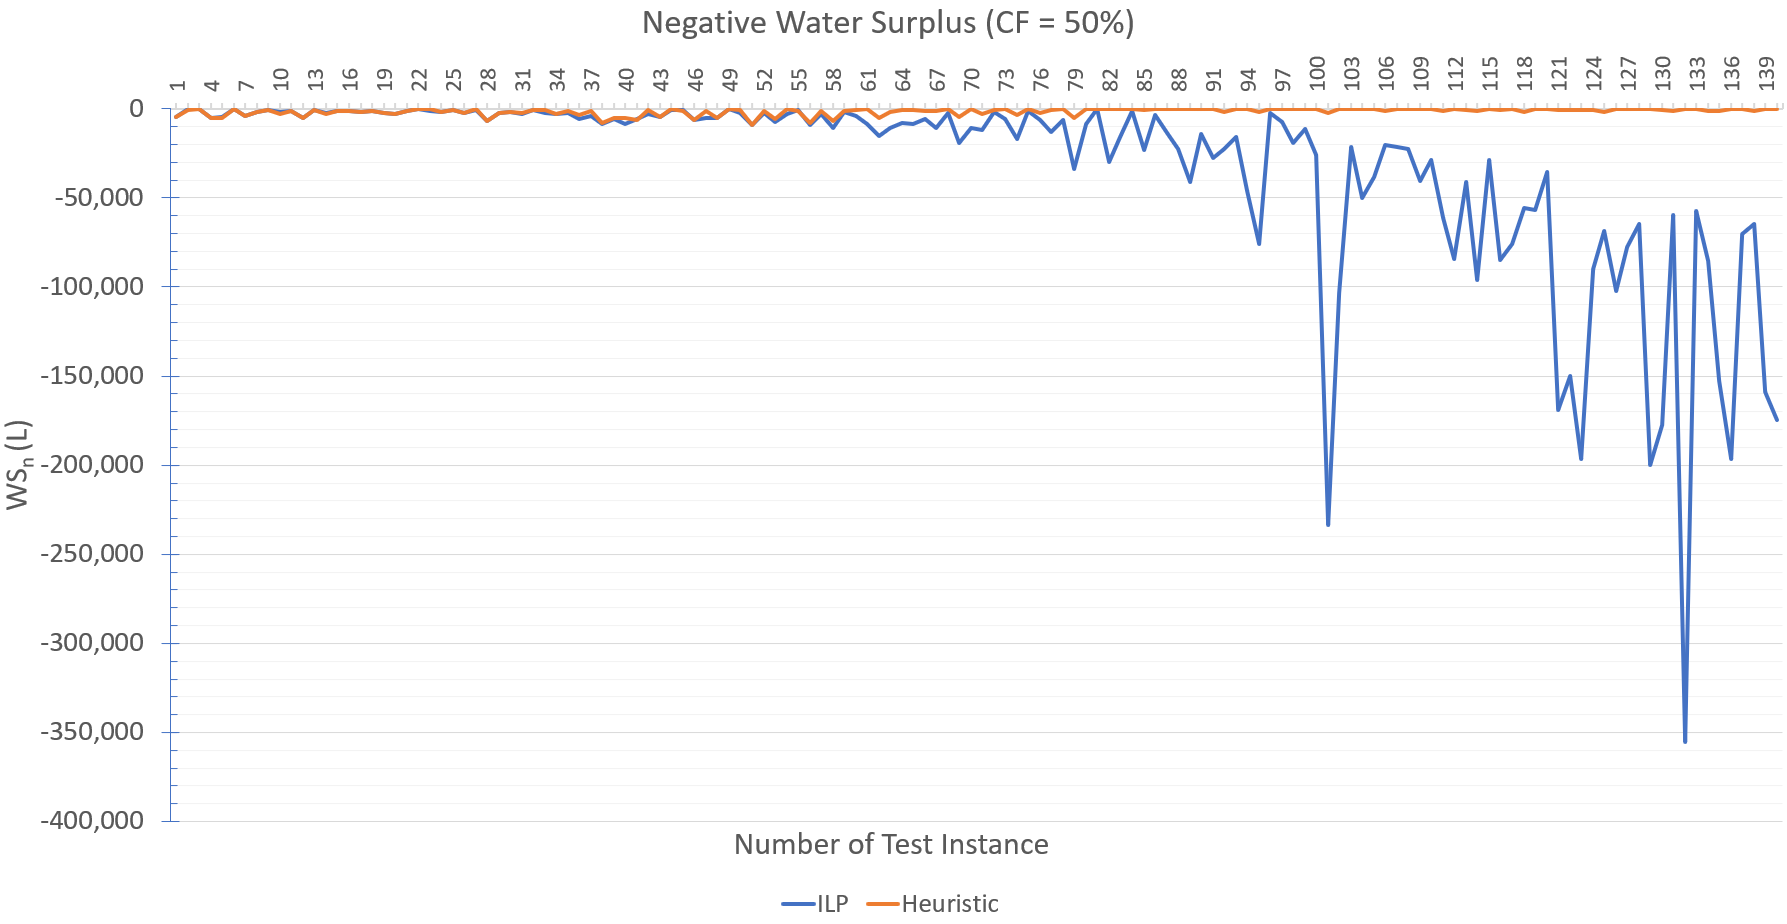
\includegraphics[width=\linewidth]{img/wsn-cf50.png}
    \caption{Comparison of negative water surplus per test instance for $\mathit{CF} = 50\%$}
    \label{fig:wsn-cf50}
\end{figure}

To get a better idea of the obtained results, Figure~\ref{fig:wsn-cf50} depicts the negative water surplus in the solutions obtained by the heuristic and ILP approaches, for each $\mathit{CF} = 50\%$ test instance.
The 140 test instances are ordered by increasing size, as if Table~\ref{tbl:comparison-cf-50} were read row by row, with the size increasing every 20 instances.
Note the scale on the vertical axis -- the negative water surplus of ILP solutions reaches hundreds of thousands of liters, while heuristic solutions stay firmly within ten thousand liters (corresponding to 2--3 drops for airtankers or heavy helicopters, or around 10 drops for light helicopters).

The relative optimality gap in CPLEX was set to $10^{-4}$, meaning that it is unlikely $\mathit{WO}$ will be optimal as it barely had any effect on the value of the objective function, and, if the absolute value of $\mathit{WS_n}$ is large, $\mathit{Z}$ might also be suboptimal, but should be fairly close.
This is the reason why, in some rare cases, the heuristic algorithm can find a better solution than what CPLEX considers to be optimal.
For example, the K07\_F02 UOF + MUOT scenarios for $\mathit{CF} = 15\%$ and $\mathit{CF} = 50\%$, and the K07\_F02 NUOF + MUOT $\mathit{CF} = 25\%$ scenario.
It is also possible that the heuristic algorithm found some optimal solutions which the ILP approach did not manage to find, however, we cannot know that for sure.

Instances with a higher $\mathit{CF}$ value have approximately uniformly higher target water content per time slot than those with a lower value.
Having very little negative water surplus in instances with a high $\mathit{CF}$ value is much more important, as it means a more uniform distribution of water was achieved for a similar total water output.
However, setting a very high $\mathit{CF}$ value (e.g., $90\%$) leads to very large absolute values of negative water surplus because it is impossible to schedule resources such that the targets are close to being satisfied.
This also often results in a large absolute value of minimal water surplus, sometimes completely ignoring several time slots, and entirely missing the goal of achieving a continuous flow of water.
As can be seen from Table~\ref{tbl:comparison-cf-50}, approximately $\mathit{CF} = 50\%$ seems to be a reasonable choice because the negative water surplus is often very close to zero.
Of course, in real-world scenarios the incident commander determines the required target water content, but their decision should be grounded on similar principles so as not to lead to unsatisfying solutions.
It should also be noted that the heuristic algorithm outperforms the ILP approach by a growing margin as $\mathit{CF}$ increases, as well as beginning to outperform ILP for smaller instances.

There seems to very little difference in solution quality for different target water content distributions over time and fronts, indicating that the heuristic algorithm is robust.
The differences are not consistent, and the relative performance for a certain distribution changes for different $\mathit{CF}$ values and scenario sizes.
This is likely due to the random nature of the test scenarios.
Perhaps some groups of scenarios had slightly higher targets and simulated worse flying conditions (reduced number of drops per hour), resulting in relatively worse solution quality.

As expected, local search always improves the solutions found by the randomized greedy algorithm.
It should be noted that, for $\mathit{CF} = 50\%$ and scenarios with 20 or more aerial resources, the greedy algorithm manages to beat the ILP approach in averaged objective values.
More precisely, it beats the ILP solutions in 72 of the 80 test instances.

For larger test instances, the randomized greedy algorithm takes approximately a third of the total execution time.
Of course, the exact ratio depends on the duration of the local search, i.e., the number of iterations $L$.
For smaller instances, the greedy algorithm finishes practically instantly.

Unfortunately, the performance of the heuristic algorithm does not improve linearly with the number of used threads.
Employing more threads, up to the number of available cores, will increase the number of performed GRASP iterations per unit of time, but will also slow down individual iterations, increasing their duration.
Therefore, the durations shown in Table~\ref{tbl:iteration-time} depict the worst-case scenario, and allow for realistic calculations of what the execution time would be for a large number of threads and iterations.
For example, for K35\_F05, 200 GRASP iterations, and 20 threads, each thread would execute 10 GRASP iterations, resulting in an execution time of approximately \SI{146}{\second}.
If a CPU with eight threads were used, it can be expected that the execution would take \SI{366}{\second}, or approximately six minutes, assuming that the processor has similar single-threaded performance as the 3900X.
If a single worker thread were used, the GRASP iteration duration would be reduced by approximately $35\%$ (measured for K35\_F05), bringing the time down to about \SI{9.5}{\second} per iteration.
Of course, it is more beneficial to perform more GRASP iterations in a predetermined amount of time, which is why using as many worker threads as reasonably possible is recommended.
In most cases, the number of worker threads should be equal to the number of logical processors.

Rudimentary testing was performed on instances outside of the scope of the defined test scenarios.
Specifically, test instances with 50 aerial resources, five fire fronts, and $\mathit{CF} = 50\%$ were used.
For the same parameters as in Table~\ref{tbl:iteration-time}, an average GRASP duration took approximately \SI{25.2}{\second}, divided into \SI{14.8}{\second} for the randomized greedy algorithm, and \SI{10.4}{\second} for local search.

Not only is the heuristic algorithm very fast, but it also uses very little memory (RAM).
For largest tested instances (K35\_F05), it reported using approximately $\SI{1}{\mega\byte} + w \cdot \SI{0.5}{\mega\byte}$ of memory, where $w$ is the number of worker threads in a thread pool.
On the other hand, the ILP approach occasionally used more than \SI{900}{\mega\byte} of RAM with 16 active threads.
With respect to the CPU usage, the number of worker threads can be specified for both approaches, making them scalable with the number of CPU cores, and therefore tied in that regard.

Table~\ref{tbl:comparison-extended} provides a comparison of ILP solutions found after six hours using a more powerful CPU, and the solutions found by the heuristic algorithm.
It can be seen that, in most cases, the heuristic algorithm will still prevail in quality, doing so in mere seconds per GRASP iteration.
ILP solutions have higher quality only for smaller instances and $\mathit{CF} = 15\%$, which is less important, and it is truly not a significant difference.
It most certainly does not justify the required execution time.
To reiterate, the heuristic algorithm found the solutions shown in Table~\ref{tbl:comparison-extended} in less than 150 seconds per problem instance (elapsed real time), on the same hardware where the linear solver was executed.
Each instance with 15 or 20 resources was solved within one minute.


\section{Hyperparameter Values}

Detailed analysis of the effects of hyperparameter values (function arguments in Algorithm~\ref{alg:grasp}) was not conducted.
From rudimentary testing it was concluded that very different values of parameters still perform remarkably well.
Also, performance depends on the specific instance -- some values might achieve better results with one instance, and worse with another.
Default values, as shown in Table~\ref{tbl:cli}, have been found to work quite well.

Generally speaking, higher numbers of GRASP and local search iterations may lead to better solutions, with diminishing returns after approximately $100$ and $7\,000$ iterations, respectively, depending on the instance size.
In some smaller instances, optimal solutions were found withing a dozen GRASP iterations.
For small instances, a couple thousand local search iterations should be more than enough.
Obviously, a larger number of iterations will increase the execution time, doing so approximately linearly.

As a rule of thumb, $N_D - N_R \le 2$ should hold.
Otherwise, the search will be slowed down significantly due to the extensive use of optimal depth-first search, with a minimal benefit to the solution quality.
It would be better to spend the time on executing more iterations than on deepened DFS.
If DFS wants to be completely avoided, the hyperparameters can be set such that $N_R \gg N_D$.

The optimal starting temperature heavily depends on the values of the weighting factors in the objective function, and the expected negative water surplus, which in turn define the expected values of the objective function.
In practice, it is a good idea to initially have approximately $50\%$ chance of accepting non-improving solutions, resulting in $T_0 \approx -1.5 \, \cdot \, \Delta f$.
The expected average value of $\Delta f$ is an open question, and depends on the problem instance.
It should not be a big issue if $T_0$ is larger than described, as that will only result in a more randomized search at the beginning, which is not necessarily a bad thing.
After $L$ local search iterations, the final temperature will be $T_L = \beta ^ L \cdot T_0$.
If one already has a final temperature in mind, the equation can be reversed in order to calculate the required cooling factor: $\beta = \log_L \left( T_L \, / \, T_0 \right)$.
If $a_1 \gg a_2 \gg a_3$ holds, and the target water content can be almost satisfied for a particular problem instance, then $T_L \in [ a_3, a_2 ]$ is a reasonable target value for the final temperature.

Weighting factors used in the greedy construction phase and the repair method ($k_{r, G}, k_{p, G}, k_{r, R}, k_{p, R}$) are particularly prone to noticeably altering the solution quality when modified.
For some instances smaller values work best, and for others it is beneficial to set them to values upwards of $10$, completely overshadowing the objective function (Algorithm~\ref{alg:greedy}, line~\ref{alg:greedy-line-fitness-def}).
Factors $k_{p, G}$ and $k_{p, R}$ should not be set close to zero if $N_R \not\gg N_D$, as that can lead to intermediate schedules which have a lot of unscheduled flights when compared to the maximum possible number of takeoffs, resulting in DFS significantly slowing down the entire search because the search depth will be much larger than expected.
If some GRASP iterations seem to take much longer than others, it might be due to DFS, and increasing $N_D$ should help resolve that problem.

Considering that a GRASP iteration can be performed within seconds, even in case of largest test instances, it is a good idea to restart the search multiple times, each time using different parameters.
Using a CPU with eight logical processors, a test scenario with 20 aerial resources can be solved ten times over within ten minutes, each time executing almost a hundred GRASP iterations.
This way, the heuristic algorithm will be used to its full potential.
